We compare the performances of our algorithm with the parallel eigenvalue problem solver SLEPc.
We compute the same amount of eigenvalues with the same number of processors using the provided Krylov-Schur algorithm \cite{stewart_krylovschur_2002}.
The performances of SLEPc in comparison of our method:

\begin{figure}[H]
  \centering
  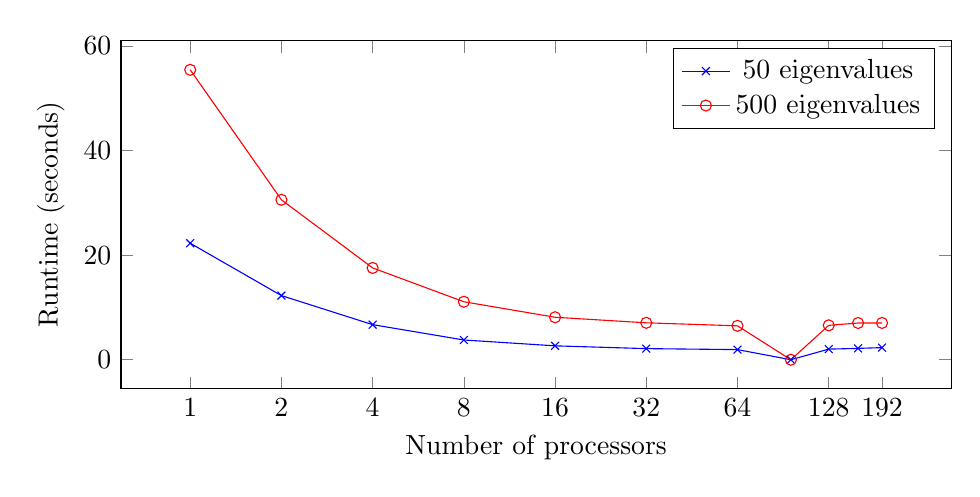
\begin{tikzpicture}
 \begin{axis}[
  height=6cm,
  width=\textwidth,
  xlabel=Number of processors,
  xtick={1, 2, 4, 8, 16, 32, 64, 128, 192},
  xmode=log,
  log ticks with fixed point,
  ylabel=Runtime (seconds)]
   \addplot[color=blue, mark=x] coordinates {
    (1, 22.2659924)
    (2, 12.2595888)
    (4, 6.7051142)
    (8, 3.7737956)
    (16, 2.6544356)
    (32, 2.1228378)
    (64, 1.9344542)
    (96, 0)
    (128, 2.027464)
    (160, 2.1684376)
    (192, 2.3157606)
   };
   \addlegendentry{50 eigenvalues}
   \addplot[color=red, mark=o] coordinates {
    (1, 55.4115932)
    (2, 30.5698838)
    (4, 17.5465694)
    (8, 11.081354)
    (16, 8.1181468)
    (32, 7.0558288)
    (64, 6.4795788)
    (96, 0)
    (128, 6.5703108)
    (160, 7.0204188)
    (192, 7.0297304)
   };
   \addlegendentry{500 eigenvalues}
 \end{axis}
\end{tikzpicture}

  \caption{Runtime of the Krylov-Schur algorithm in SLEPc (log scale).}
\end{figure}

First of all, it is notable that both execution times for 50 and 500 eigenvalues are close to each other.
This comes from the way the internal Krylov-Schur algorithm functions.
Also, we observe that both plots have the same profile and evolve in the same way with respect to the number of processors.
%It has to compute multiple eigenpairs and then discard the unwanted ones, meaning that the method can have the same performances for different amounts of requested eigenvalues.

The algorithm, on this test case, is faster than our implementation.
However, both approaches tend to have a light increase in the runtime after reaching a certain number of processors.
